% ETF Factsheet Template — edit and compile online at https://letx.app
% Compiles clean with: latexmk -pdf main.tex
\documentclass[11pt,a4paper]{article}

% ── Encoding & Font ──────────────────────────────────────────────────
\usepackage[T1]{fontenc}
\usepackage{lato}
\renewcommand{\familydefault}{\sfdefault}

% ── Core packages ────────────────────────────────────────────────────
\usepackage{amsmath}
\usepackage[margin=1.6cm, top=2.6cm, bottom=1.8cm, headheight=14pt]{geometry}
\usepackage[table]{xcolor}
\usepackage{booktabs}
\usepackage{tabularx}
\usepackage{ragged2e}
\usepackage{multirow}
\usepackage{enumitem}
\usepackage[most]{tcolorbox}
\tcbuselibrary{skins,breakable}
\usetikzlibrary{shadows}
\usepackage{tikz}
\usepackage{pgfplots}
\pgfplotsset{compat=1.18}
\usepackage{fontawesome5}
\usepackage{titlesec}
\usepackage{caption}
\usepackage{fancyhdr}
\usepackage{hyperref}

% ── TikZ libraries ───────────────────────────────────────────────────
\usetikzlibrary{shadows, arrows.meta, positioning, calc, backgrounds}

% ── Colour palette ───────────────────────────────────────────────────
\definecolor{navy}{HTML}{1B2A4A}
\definecolor{gold}{HTML}{C8963E}
\definecolor{slate}{HTML}{6B7D8E}
\definecolor{ice}{HTML}{F4F6F9}
\definecolor{darkgreen}{HTML}{2D7D46}
\definecolor{warning}{HTML}{D4A017}

% ── Section formatting ───────────────────────────────────────────────
\titleformat{\section}
  {\Large\bfseries\color{navy}}
  {}
  {0pt}
  {}
  [\vspace{-0.5em}\textcolor{gold}{\rule{\linewidth}{1.2pt}}\vspace{0.3em}]
\titlespacing{\section}{0pt}{1.2em}{0.6em}

\titleformat{\subsection}
  {\large\bfseries\color{navy!80}}
  {}
  {0pt}
  {}
\titlespacing{\subsection}{0pt}{0.8em}{0.3em}

% ── Spacing ──────────────────────────────────────────────────────────
\setlength{\parindent}{0pt}
\setlength{\parskip}{0pt}
\setlength{\tabcolsep}{6pt}
\renewcommand{\arraystretch}{1.15}

% ── Fancyhdr ─────────────────────────────────────────────────────────
\pagestyle{fancy}
\fancyhf{}
\renewcommand{\headrulewidth}{0pt}
\fancyfoot[L]{\footnotesize\color{slate}Meridian Asset Management \textbar\ For professional clients only}
\fancyfoot[R]{\footnotesize\color{slate}\thepage}

% ── Helper commands ──────────────────────────────────────────────────
\newcommand{\keyvaltable}[1]{%
  \bgroup
  \setlength{\parindent}{0pt}%
  \setlength{\parskip}{0pt}%
  \renewcommand{\arraystretch}{1.35}%
  \begin{tabularx}{\linewidth}{@{}>{\color{navy}\bfseries}l@{\hspace{6mm}}>{\raggedright\arraybackslash}X@{}}
    #1
  \end{tabularx}%
  \egroup
}

\newtcolorbox{factbox}[1][]{
  colback=ice,
  colframe=navy!20,
  arc=4pt,
  boxrule=0.6pt,
  left=10pt,
  right=10pt,
  top=8pt,
  bottom=8pt,
  before skip=8pt,
  after skip=8pt,
  #1
}

\newtcolorbox{statcard}[1][]{
  colback=navy,
  colframe=navy,
  arc=6pt,
  boxrule=0pt,
  left=10pt,
  right=10pt,
  top=8pt,
  bottom=8pt,
  before skip=4pt,
  after skip=4pt,
  fontupper=\color{white},
  #1
}

\newcommand{\statval}[1]{{\fontsize{22}{26}\selectfont\bfseries\color{gold}#1}}
\newcommand{\statlabel}[1]{{\footnotesize\color{white!85}#1}}

\newcommand{\esgbar}[1]{%
  \begin{tikzpicture}[baseline=(current bounding box.center)]
    \fill[ice] (0,0) rectangle (5.5,0.28);
    \fill[navy] (0,0) rectangle (#1*0.55,0.28);
  \end{tikzpicture}%
}

% ── Title / header bar ───────────────────────────────────────────────
\newcommand{\printheader}{%
  \begin{tikzpicture}[remember picture, overlay]
    \fill[navy] (current page.north west) rectangle ([yshift=-2.3cm]current page.north east);
    \fill[gold] (current page.north west) rectangle ([yshift=-2.38cm]current page.north east);
    \node[anchor=south west, text=white, font=\LARGE\bfseries]
      at ([xshift=1.2cm, yshift=-0.75cm]current page.north west)
      {Meridian Core US 500 UCITS ETF};
    \node[anchor=south west, text=white!80, font=\small]
      at ([xshift=1.2cm, yshift=-1.35cm]current page.north west)
      {Ticker: MER5 \textbar\  ISIN: IE00BMERID50 \textbar\  Exchange: London Stock Exchange};
    \node[anchor=south west, text=white!60, font=\footnotesize]
      at ([xshift=1.2cm, yshift=-1.85cm]current page.north west)
      {Domicile: Ireland \textbar\  Income: Accumulating \textbar\  Base Currency: USD \textbar\  TER: 0.07\%\ p.a.};
  \end{tikzpicture}%
  \vspace*{2.6cm}%
}

\begin{document}

\printheader

% ═══════════════════════════════════════════════════════════════════════
%  PAGE 1 — FUND OVERVIEW
% ═══════════════════════════════════════════════════════════════════════

% ── Two-column top section ───────────────────────────────────────────
\noindent
\begin{minipage}[t]{0.62\linewidth}

\section{Fund Objective}

The Meridian Core US 500 UCITS ETF seeks to track the investment results of an index
composed of large-capitalisation U.S. equities. The fund aims to provide investors with
cost-efficient, liquid access to the Meridian US 500 Index, a
market-capitalisation-weighted index of 500 leading publicly traded companies in the
United States.

\vspace{6pt}

\subsection*{Index Replication Methodology}

\begin{center}
\resizebox{\textwidth}{!}{%
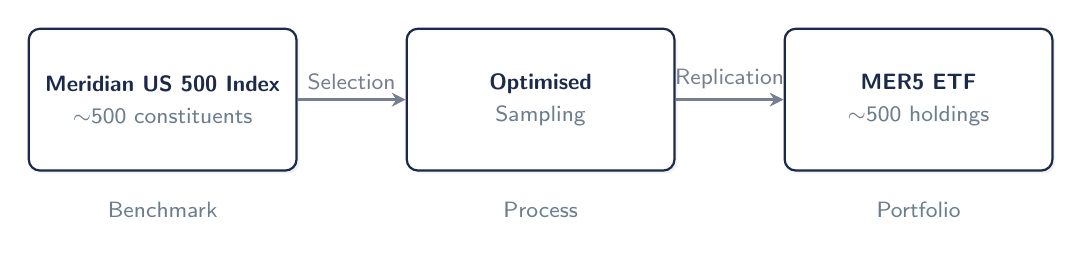
\begin{tikzpicture}[
    box/.style={
      draw=navy, fill=white, rounded corners=4pt,
      minimum width=3.4cm, minimum height=1.8cm,
      align=center, font=\footnotesize\bfseries, text=navy,
      line width=0.8pt, drop shadow={shadow xshift=1pt, shadow yshift=-1pt, opacity=0.12}
    },
    arrow/.style={-{Stealth[length=5pt, width=5pt]}, navy!60, line width=1pt},
    label/.style={font=\footnotesize\color{slate}, align=center}
  ]
  \node[box] (index) at (0,0) {Meridian US 500 Index\\[2pt]{\normalfont\footnotesize\color{slate}$\sim$500 constituents}};
  \node[box] (method) at (4.8,0) {Optimised\\[2pt]{\normalfont\footnotesize\color{slate}Sampling}};
  \node[box] (etf) at (9.6,0) {MER5 ETF\\[2pt]{\normalfont\footnotesize\color{slate}$\sim$500 holdings}};

  \draw[arrow] (index.east) -- (method.west)
    node[midway, above, font=\footnotesize\color{gold}]{Selection};
  \draw[arrow] (method.east) -- (etf.west)
    node[midway, above, font=\footnotesize\color{gold}]{Replication};

  \node[label] at (0,-1.4) {Benchmark};
  \node[label] at (4.8,-1.4) {Process};
  \node[label] at (9.6,-1.4) {Portfolio};
\end{tikzpicture}}
\end{center}

\vspace{4pt}
{\footnotesize\color{slate}
The fund uses a sampling technique to replicate the index. It holds a representative subset
of securities that collectively mirrors the risk and return profile of the Meridian US 500, minimising
tracking error while maintaining cost efficiency.}
\end{minipage}%
\hfill
\begin{minipage}[t]{0.35\linewidth}

\vspace{-0.4em}
\begin{statcard}
  \centering
  \statval{\$85.2\,B}\\[2pt]
  \statlabel{AUM as of 30 Jun 2026}

  \vspace{6pt}
  \statval{0.07\%}\\[2pt]
  \statlabel{Total Expense Ratio}

  \vspace{6pt}
  \statval{18 May 2010}\\[2pt]
  \statlabel{Inception Date}

  \vspace{6pt}
  \statval{\faChartBar\ \ 7.5\,M}\\[2pt]
  \statlabel{30-Day Avg.\ Volume}
\end{statcard}

\vspace{8pt}

\begin{factbox}
\footnotesize
\keyvaltable{
  Index Ticker              & MRX500 \\
  Number of Holdings        & 503 \\
  Price/Earnings Ratio      & 22.4$\times$ \\
  Price/Book Ratio          & 4.6$\times$ \\
  Dividend Yield            & 1.32\,\% \\
  Distribution Frequency    & Semi-Annual \\
  Share Class Currency      & USD \\
  Use of Income             & Accumulating \\
  Securities Lending        & Yes (max 30\,\%) \\
}
\end{factbox}

\end{minipage}

\vspace{4pt}

% ── Top 10 Holdings ──────────────────────────────────────────────────
\section{Top 10 Holdings}
\noindent
\renewcommand{\arraystretch}{1.25}
\begin{tabularx}{\linewidth}{
  @{}>{\columncolor{ice!60}}l
  l
  >{\raggedleft\arraybackslash}X
  >{\raggedleft\arraybackslash}X
  @{}}
\toprule
\rowcolor{navy}
\color{white}\bfseries \# &
\color{white}\bfseries Name &
\color{white}\bfseries Weight &
\color{white}\bfseries Sector \\
\midrule
1 & Apex Technologies Inc.                     & 7.21\,\% & Information Technology \\
2 & Nimbus Software Corp.          & 6.84\,\% & Information Technology \\
3 & Vertex Commerce, Inc.               & 3.92\,\% & Consumer Discretionary \\
4 & Quanta Silicon Corp.             & 3.47\,\% & Information Technology \\
5 & Lumina Holdings (Class A)        & 2.28\,\% & Communication Services \\
6 & Synapse Social, Inc.           & 2.14\,\% & Communication Services \\
7 & Lumina Holdings (Class C)        & 1.98\,\% & Communication Services \\
8 & Keystone Capital Inc.        & 1.72\,\% & Financials \\
9 & Halcyon Semiconductors Inc.                  & 1.53\,\% & Information Technology \\
10& Helios Motors, Inc.                    & 1.38\,\% & Consumer Discretionary \\
\midrule
\multicolumn{2}{l}{\bfseries\color{navy} Top 10 Aggregate}
  & \bfseries\color{navy} 32.47\,\% & \\
\bottomrule
\end{tabularx}
\captionsetup{font={footnotesize,color=slate}, labelformat=empty}
\captionof{table}{Weights as of 30 Jun 2026. Holdings subject to change.}

\newpage

% ═══════════════════════════════════════════════════════════════════════
%  PAGE 2 — RISK \& ESG
% ═══════════════════════════════════════════════════════════════════════

\printheader

% ── Sector Breakdown ─────────────────────────────────────────────────
\section{Sector Breakdown}

\noindent
\begin{minipage}[t]{0.56\linewidth}
\vspace{-0.4em}
\resizebox{\textwidth}{!}{%
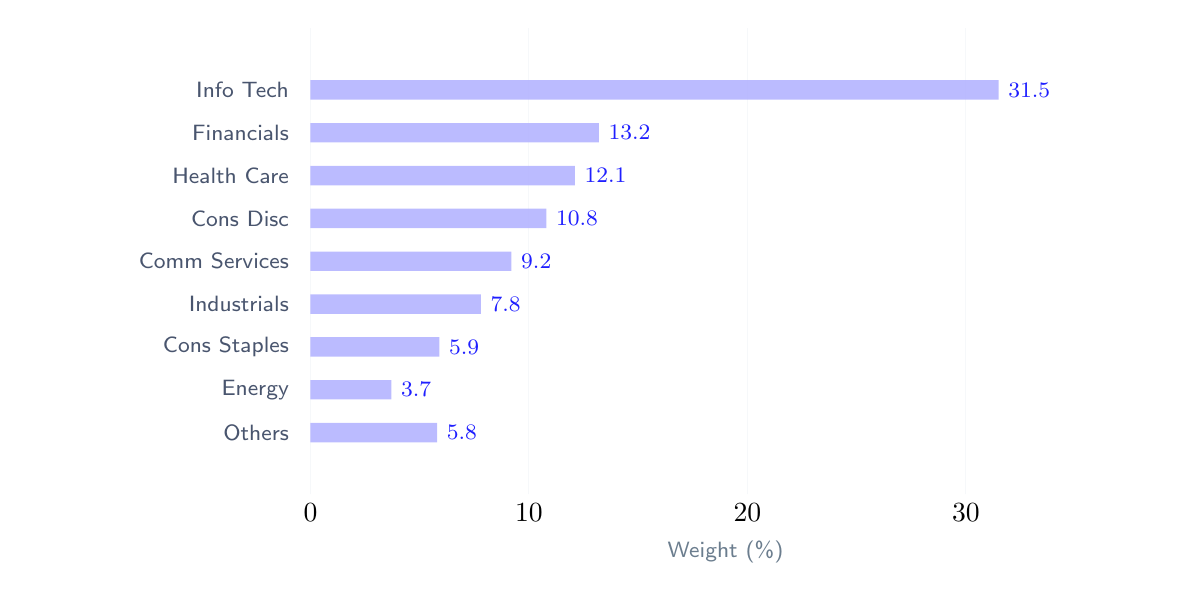
\begin{tikzpicture}
\begin{axis}[
  xbar,
  width=\linewidth,
  height=7.5cm,
  bar width=7pt,
  enlarge y limits=0.18,
  xmin=0, xmax=38,
  symbolic y coords={
    Others, Energy, Cons Staples, Industrials,
    Comm Services, Cons Disc, Health Care, Financials, Info Tech
  },
  ytick=data,
  y tick label style={font=\footnotesize\color{navy!80}, align=right, text width=3.2cm},
  xlabel={Weight (\%)},
  xlabel style={font=\footnotesize\color{slate}},
  nodes near coords,
  nodes near coords style={font=\footnotesize\color{navy}, /pgf/number format/precision=1},
  nodes near coords align={horizontal},
  axis line style={draw=none},
  tick style={draw=none},
  xtick={0,10,20,30},
  xtick style={draw=ice!80, thin},
  major grid style={ice!80, thin},
  xmajorgrids=true,
  every axis plot/.append style={fill=navy, draw=none, opacity=0.88}
]
\addplot coordinates {
  (31.5,Info Tech)
  (13.2,Financials)
  (12.1,Health Care)
  (10.8,Cons Disc)
  (9.2,Comm Services)
  (7.8,Industrials)
  (5.9,Cons Staples)
  (3.7,Energy)
  (5.8,Others)
};
\end{axis}
\end{tikzpicture}}
\end{minipage}%
\hfill
\begin{minipage}[t]{0.40\linewidth}

\vspace{0.4em}
\begin{factbox}
\footnotesize
\keyvaltable{
  \faGlobe\ \ Top Sector     & Information Technology (31.5\%) \\
  \faGlobe\ \ 2nd Sector     & Financials (13.2\%) \\
  \faGlobe\ \ Top 3 Weight   & 56.8\,\% \\
  \faGlobe\ \ Concentration  & Moderate (HHI: 0.052) \\
}
\end{factbox}

\vspace{6pt}
{\footnotesize\color{slate}
The fund's sector allocation closely mirrors the Meridian US 500 benchmark. Information Technology
dominates, reflecting the index's market-cap weighting. Sector deviations from the benchmark
are maintained within $\pm$0.25\,\% to minimise active risk.}

\end{minipage}

\vspace{2pt}

% ── Risk Metrics ─────────────────────────────────────────────────────
\section{Risk Metrics}

\noindent
\renewcommand{\arraystretch}{1.3}
\begin{tabularx}{\linewidth}{
  @{}>{\columncolor{ice!60}\bfseries\color{navy}}l
  X
  >{\centering\arraybackslash}p{2.2cm}
  >{\centering\arraybackslash}p{2.2cm}
  >{\centering\arraybackslash}p{2.2cm}
  @{}}
\toprule
\rowcolor{navy}
\color{white}\bfseries Metric &
\color{white}\bfseries Description &
\color{white}\bfseries 1 Year &
\color{white}\bfseries 3 Year &
\color{white}\bfseries 5 Year \\
\midrule
Standard Deviation    & Annualised volatility of NAV returns  & 14.8\,\% & 17.2\,\% & 18.1\,\% \\
Sharpe Ratio          & Excess return per unit of risk (RFR: 4.5\%) & 1.12  & 0.68  & 0.74  \\
Maximum Drawdown      & Largest peak-to-trough decline          & $-$8.2\,\% & $-$23.9\,\% & $-$23.9\,\% \\
Beta                  & Sensitivity to benchmark (Meridian US 500)     & 1.00  & 1.00  & 1.00  \\
Tracking Error        & Std.\ dev.\ of excess returns vs.\ benchmark & 0.04\,\% & 0.05\,\% & 0.06\,\% \\
Information Ratio     & Excess return per unit of tracking error & 0.18  & 0.12  & 0.09  \\
VaR (95\%, 1-month)   & Value at Risk (historical simulation)    & $-$5.6\,\% & $-$6.4\,\% & $-$6.8\,\% \\
Sortino Ratio         & Downside-risk-adjusted return            & 1.64  & 0.98  & 1.03  \\
Upside Capture        & Performance in up markets vs.\ benchmark & 99.8\,\% & 99.6\,\% & 99.5\,\% \\
Downside Capture      & Performance in down markets vs.\ benchmark & 100.1\,\% & 100.3\,\% & 100.4\,\% \\
\bottomrule
\end{tabularx}
\captionsetup{font={footnotesize,color=slate}, labelformat=empty}
\captionof{table}{Risk metrics calculated using monthly returns. Source: Meridian Asset Management, as of 30 Jun 2026.}

\vspace{4pt}

% ── ESG Profile ──────────────────────────────────────────────────────
\section{ESG Profile}

\noindent
\begin{minipage}[t]{0.48\linewidth}

\vspace{2pt}
\begin{factbox}
\centering
{\large\bfseries\color{darkgreen}ESG Rating: AA}\\[4pt]
{\footnotesize\color{slate}(Scale: CCC -- B -- BB -- BBB -- A -- AA -- AAA)}
\end{factbox}

\vspace{6pt}
\keyvaltable{
  ESG Score (0--10)        & \textbf{7.8} \esgbar{7.8} \\
  Environmental Pillar     & \textbf{6.2} \esgbar{6.2} \\
  Social Pillar            & \textbf{8.1} \esgbar{8.1} \\
  Governance Pillar        & \textbf{6.9} \esgbar{6.9} \\
}

\end{minipage}%
\hfill
\begin{minipage}[t]{0.48\linewidth}

\vspace{2pt}
\subsection*{Key ESG Metrics}

\keyvaltable{
  Carbon Intensity           & 78.5 tCO\textsubscript{2}e / \$M sales \\
  \% ESG-Covered     & 99.8\,\% \\
  SFDR Classification        & Article 8 \\
  UN Global Compact Violators& 0.0\,\% \\
  Controversial Weapons Exp. & 0.0\,\% \\
  Thermal Coal Exposure      & 0.3\,\% \\
  Tobacco Exposure           & 0.0\,\% \\
}

\vspace{8pt}
{\footnotesize\color{slate}
Carbon intensity is weighted-average scope~1~+~2 emissions per million USD of sales.
Data sourced from internal ESG research. SFDR = EU Sustainable Finance Disclosure Regulation.}

\end{minipage}

\vspace{6pt}

% ── Disclaimer ───────────────────────────────────────────────────────
\begin{tcolorbox}[
  colback=ice!80,
  colframe=ice!80,
  arc=2pt,
  boxrule=0pt,
  left=8pt,
  right=8pt,
  top=6pt,
  bottom=6pt,
  before skip=8pt,
  fontupper=\fontsize{7.2}{9}\selectfont\color{slate}
]
\textbf{Disclaimer:} This document is for informational purposes only and does not constitute
investment advice, a recommendation, or an offer to buy or sell any security. Past performance
is not a reliable indicator of future results. The value of investments may fluctuate and
investors may not get back the amount originally invested. Meridian\texttrademark
is a trademark of Meridian Asset Management. This is a sample template, not a real product.
Meridian US 500 is a registered trademark of S\&P Global. All data
as of 30 June 2026 unless otherwise stated. Source: Meridian Asset Management, internal research.
For professional clients only --- not for retail distribution.
\end{tcolorbox}

\end{document}
